% File name: datalogger/Reports/Final_Report_Andy.tex
% Final report for datalogger project
% Author: adh
% Date: Mon 03 Jun 2013 11:51

\documentclass[a4paper,10pt]{article}  % Standard document class
\usepackage[english]{babel}            % Set document language
\usepackage{fullpage}                  % Set up page for small margins etc

\usepackage{todonotes}

\usepackage{graphicx}                  % For including images in document
\usepackage{placeins}                  % Allows use of \FloatBarrier
% to avoid images or tables
% moving into next section
\usepackage{subfig}                    % For subfigures...

\usepackage{amsmath}                   % For improving maths/formula typesetting
\usepackage{tabularx}                  % Table changing package

\usepackage{algpseudocode}             % For producing algorithms/flowcharts
\usepackage{listings}                  % For including source code in document

\usepackage{url}

% Provide command for scientific notation
\providecommand{\e}[1]{\ensuremath{\times10^{#1}}}
\providecommand{\degrees}{\ensuremath{^{\circ}}}

% Define title here:
\title{Project SB3: Data Logger\\
       Package Environment Monitoring\\
       Final Report}
\author{Andrew Holt\\
        ah635\\
        Team 6\\
        Emmanuel}
\date{06 June 2013}

\begin{document}

\listoftodos

% generate title
\maketitle

\begin{center}
  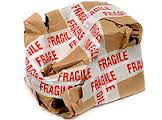
\includegraphics[width=0.3\textwidth]{damaged_parcel.jpg}
\end{center}

\noindent summary: motive, method, key results, conclusions \todo{add summary/abstract}

\tableofcontents

\section{Introduction}
\label{sec:introduction}

The express delivery industry is one of the fastest growing industries
in the world today. In 2003, the industry made a direct contribution
of US\$64 billion to worldwide GDP, and has been growing by around 8\%
per year since \cite{OEF2005}. However, customers have very little
information of the environmental and handling conditions their package
has been subject to during its transit. When shipping fragile or
sensitive products, the conditions that the parcel is subject to may
be critical in the integrity of the product. The two major issues here
are:
\begin{enumerate}
\item Fragile goods which arrive broken: it is desirable to determine
  whether the package has been mishandled, and if so by whom.
\item Perishable goods: if they have been subjected to conditions
  outside of sensitive temperature and humidity limits they will have
  a shorted shelf life. This may not be obvious upon inspection of the
  goods, so detailed condition tracking is required.
\end{enumerate}
While products have been around for a while to carry out this type of
tracking on shipping containers, the same problem applies to smaller
and domestic packages too. In the past six months, two large companies
have announced products to achieve this, but it is clearly an emerging
market and a good product launched now could have a great chance of
success. One of these, ``SenseAware''\cite{SA_PR} by FedEx
Corporation, is already released and availiable however this is only
available on a select number of carriers and services and is a
business level product, not suited for everyday or relatively low
value package monitoring. An alternative is the ``DropTag'' system
recently announced by Cambridge Consultants \cite{DT_PR}, however this
system is not yet at the commercial release stage.

With a problem identified and a solution required, as well as a clear
business opportunity due to the interest in development from other
companies, product development was begun.

\section{Overview}
\label{sec:overview}

In order to effectively track the condition of a parcel during
transit, the final product was clearly required to be cheap, low power
and physically small and robust. For this project, a simple prototype
was to be developed, which if successful could be miniaturised and
fabricated for the final product.

\subsection{Summary of Design}
\label{sec:summary-design}

The first stage of the design process was to evaluate which quantities
should be measured and logged. The key environmental variables would
be temperature and humidity. Vibration, orientation and shocks would
also be required to understand the handling and transport
conditions. GPS tracking would also be useful, but it was decided to
focus on the other five initially as GPS could be relatively easily
included with a dedicated GPS chip communicating over the I$^2$C
protocol, and GPS reception may be limited at many points during
transit.

The product would clearly be required to work without being plugged in
to a computer, so a standalone mode would be developed. It would be
useful for development, debugging and testing to operate with instant
feedback from the computer system, so a linked mode was also
developed.

To ensure long term operation, on-board memory would be required, so an
EEPROM was used for data storage in the standalone mode. This would
also require a battery supply.

Some kind of on-board display would also be useful on the board, for
monitoring, debugging and status display, so an LCD screen was used
along with five LEDs.

The platform choices were specified in the project requirements, so
the project was to be developed for the STM32F100 ARM Cortex MCU and a
PC running the Windows operating system. The key design areas would
therefore be hardware, firmware and software. The budget was generous
for the development board so cost was not really an issue, however to
achieve a commercial product, the cost and size would need to be
reduced. This could be achieved by miniaturising, as surface mount
components tend to be cheaper; and use of a cheaper MCU (which wouldn't
need the development features of the STM).

The project block diagram is shown in figure \ref{fig:sysblkdgrm}.
\begin{figure}[htb]
  \begin{center}
    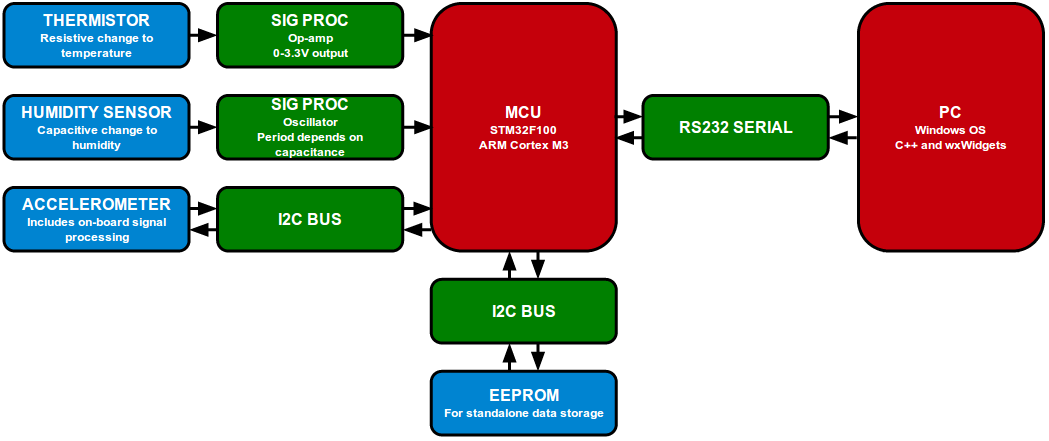
\includegraphics[width=1.0\textwidth]{System_diagram.png}
  \end{center}
  \caption{Overall system block diagram}
  \label{fig:sysblkdgrm}
\end{figure}

\subsection{Project Management}
\label{sec:project-management}

The project was divided between the two team members. It was decided
that James would write the firmware for the MCU, Andrew would write
the software for the computer and the hardware design was to be
shared. The general development plan was to start by making a basic
but working system and gradually adding features and complexity upon
the existing system. This ensured that we would have a fully
operational product, if not with every desired feature, by the end of the
project, and would also allow the simpler parts to be used in testing
more complex parts.

Initally basic hardware circuits were designed and built. The firmware
and software were then developed. The hardware circuits were highly
useful in testing the firmware, but in writing the firmware, flaws in
the circuit designs became apparent, such as the initial plan to use a
simple charge-discharge of the humidity sensor. For this reason, the
humidity sensor circuit was updated during the project.

\section{Design}
\label{sec:design}

A brief overview of the design has been given in section
\ref{sec:summary-design}. This section gives technical detail about
the parts of the system which I designed. The other parts are detailed
in James' report.

\todo{add photo of completed board}

\subsection{Hardware}
\label{sec:hardware}

In order to measure temperature, it was decided to use a
thermistor. Thermistors have advantages over other temperature
measurement devices such as thermocouples, resonant crystal
thermometers and diode junction voltage measurement such as \cite{HH}: 
\begin{enumerate}
  \item The dependant quantity is very easy to measure.
  \item Large change in measured quantity (thousands of ohms, compared
    to millivolt changes in thermocouples and diode junctions), meaning
    low demands are placed on the analogue circuitry.
  \item Inexpensive.
  \item Good stability.
  \item Circuit can easily be designed to give very linear output,
    making the digital conversion to temperature straightforward.
\end{enumerate}
With these considerations, an ND06P00103K NTC $10\,\mathrm{k\Omega}$ thermistor from AVX was
selected, based on price and good electrical characteristics based on
the application requirements.

An analogue signal processing circuit was required to process the
output from the thermistor to a signal usable by the MCU
analogue-to-digital converter (ADC). This required a signal in the
range of $0-3.3\,\mathrm{V}$.

The thermistor was placed in a voltage divider circuit with a series
$10\,\mathrm{k\Omega}$ resistor. This was selected to linearize the
temperature curve. This combination gives a response linear to within
$1\,\mathrm{\%}$ from $0\ \mathrm{to}\ 40\,\mathrm{\degrees C}$ and
$3\,\mathrm{\%}$ between $-10\ \mathrm{and}\ 50\,\mathrm{\degrees
  C}$. This voltage divider operates from a 3.3V rail, ensuring that
the input to the next stage will always lie within its supply
rails. At this supply level, the maximum power dissipation through the
thermistor was calculated as $3.3\,\mathrm{mW}$ at
$50\,\mathrm{\degrees C}$. This is well below the maximum dissipation
for the thermistor of $0.71\,\mathrm{mW}$, so will not have a
noticeable affect on the temperature measurement.

The output from the voltage divider is input to an op-amp
non-inverting amplifier circuit. The voltage divider has relatively
high output resistance, so use of a non-inverting op-amp configuration
ensures a very large input resistance ($\sim 10^{13}\,
\mathrm{\Omega}$), avoiding loading on the measurement circuit.

The non-inverting amplifier is slightly non-standard due to a non-zero
reference voltage on the inverting terminal. This is selected to give
the same output as the thermistor setup at the low end of its
response, which was selected as $-20\,\mathrm{\degrees C}$ as this
will lie well below the temperature a package would expect to
experience in transit and is at the limit of the linear response. This
reference voltage was found to be $0.79\,\mathrm{V}$, so is generated
using a series combination of $22\,\mathrm{k \Omega}$ and two
$10\,\mathrm{k \Omega}$ resistors, giving a very close voltage match
with standard resistor values.

The gain was then calculated to produce a $3.3\,\mathrm{V}$ output
swing over the input range to be received, and the gain required was
found to be 1.47. This was achieved in the non-inverting amplifier
using standard resistor values of $56\ \mathrm{and}\ 120\,\mathrm{k
  \Omega}$.

The output swing was chosen to span the full supply level of
$0-3.3\,\mathrm{V}$ as the op-amp used provides very good rail-to-rail
operation, and the extremes of the working temperature range are both
unlikely to experienced and reaching the limits of the linear response
from the thermistor. For the package tracking application, it is not
critical to know how far beyond these limits the temperature has
reached, so a simple saturating output is sufficient.

The circuit diagram for the temperature monitoring circuit is shown in
appendix \ref{sec:source-code-circuit}, figure \ref{fig:tempcct}.

\subsection{Software}
\label{sec:software}

It was suggested to use the National Instruments ``LabWindows/CVI''
package for developing the PC software and graphical user interface
(gui), however it was decided to eschew this in favour of developing
in C++ and the wxWidgets cross platform gui toolkit. The reasons for
this were:
\begin{enumerate}
\item LabWindows is a highly specialist and proprietary development
  package. While it is simple to use and fast to setup, we found it
  unlikely that we would use it again in the future.
\item LabWindows is fairly limited in scope of what can be achieved,
  whereas wxWidgets and C++ allow pretty much anything to be achieved.
\item Our other project was using C++ and wxWidgets, so it was a
  simpler option to only learn one package, rather than one per project.
\item Past experience of coding in C++ could be utilised, whereas
  LabWindows relies on C which I have very little experience of.
\end{enumerate}

There are three main components to the software development. The
backend functionality required serial port communications and
communications protocols with the microcontroller. The front end required a simple
user interface to display the logged data and control the
microcontroller functions.

The actual data transmission is handled by the serial port
library.

The sending of packets to and from the serial port for the
microcontroller are handled by the communications level, which
provides an interface between the application and the actual data, so
the user and user interface level do not depend on the communications
system. This is advantageous as it means the top level application is
independent of the communication medium, and could be converted to use
USB or wifi without modifying the user application. It also simplifies
the functions required in the user application as they do not directly
handle the raw data, but instead use more user/programmer friendly
data structures.

On top of the communications layer is the application and user
interface layer. These allow easy and logical viewing and
understanding of commands to be sent and data received by the
computer.

This hierarchical structure is shown in figure
\ref{fig:commsprotocol}. The layers map very roughly onto the Open
Systems Interconnect (OSI) reference model. The user interface
performs the duties of layer 7 (application). The communications layer
is similar to layer 6 (presentation), while the rs232 library spans
levels 4 and 5 (transport and session layers, respectively). The lower
layers are defined by the RS232 protocol.

\begin{figure}[!htb]
  \begin{center}
    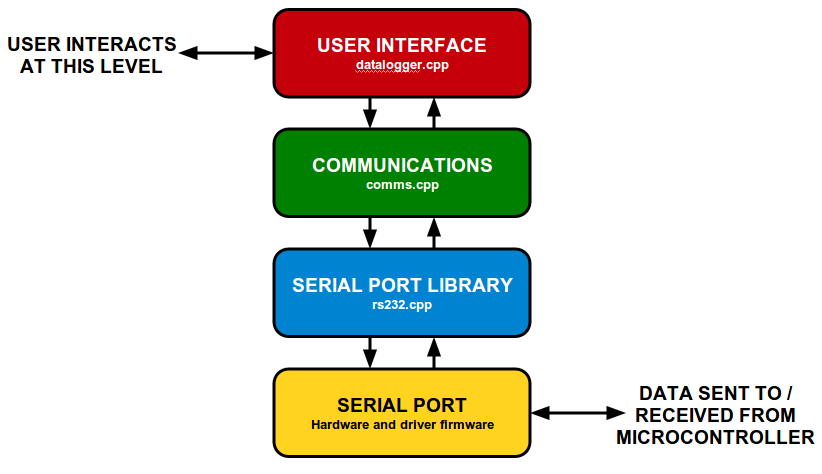
\includegraphics[width=0.7\textwidth]{CommunicationsProtocol.png}
  \end{center}
  \caption{Communications stack showing interaction of each layer.}
  \label{fig:commsprotocol}
\end{figure}

\subsubsection{Serial Port Communications}

The files \texttt{rs232.cpp} and \texttt{rs232.h} contain functions for
sending and receiving data from the serial port. These were found
online \cite{rs232_lib}, released under the GNU General Public
Licence. (See section \ref{sec:probl-enco-techn} for more details.)

The important functions provided by this software is are:
\begin{description}
  \item[\texttt{RS\_232\_OpenComport()}]
    This sets up the connection with the serial port to be used,
    setting up a two way communications link to the microcontroller.
  \item[\texttt{RS\_232\_CloseComport()}] Closes the connection to the
    serial port at the end of the operation.
  \item[\texttt{RS\_232\_PollComport()}] Reads data that has been sent
    by the microcontroller to the computer.
  \item[\texttt{RS\_232\_SendBuf()}] Writes to the serial port to send
    commands to the microcontroller.
\end{description}

These functions were all provided directly by the software found
online, which greatly simplified the serial port reading.

\subsubsection{Communications}

The functions provided in the RS\_232 library are very low level, and
perform sending and receiving of individual bytes. For the user
interface, it is useful to have a high level data structure, rather
than dealing with individual bytes of data. The files
\texttt{comms.cpp} and \texttt{comms.h} provide the means to do
this. The functions here call the functions in \texttt{rs232.cpp}. It
converts the user commands into the required bytes to send to the
microcontroller, and organises the returned data into a
\texttt{vector} data structure.

This level provides functions to be called by the datalogger
application:
\begin{description}
  \item[\texttt{RS232\_Init()}] Opens the required comport to
    establish a link with the microcontroller.
  \item[\texttt{RS232\_Close()}] Closes the opened comport.
  \item[\texttt{send\_command()}] Sends a command to the
    microcontroller by writing to the serial port buffer (uses the
    \texttt{SendBuf} function).
  \item[\texttt{read\_eeprom\_data()}] Reads data stored in the EEPROM
    into a \texttt{vector}.
  \item[\texttt{get\_Readings()}] Receives the data sent by the
    microcontroller in linked mode and stores it in a vector.
\end{description}

\subsubsection{User Interface}

The top level of the PC system is the user interface, which allows the
user to interact with the system in an intuitive and non-technical
way. The user interface is shown in figure



The user can click buttons and select values from a drop down menu to
operate the data logger. The output from the monitoring is displayed
directly on the screen during the 

\subsection{Communications}

\section{Problems Encountered and Technical Solutions}
\label{sec:probl-enco-techn}

require rs232 library since couldn't use LabWindows one.

display of data: csv output \& plotting in python/excel.

running logging in background while allowing gui functionality.

accelerometer, humidity sensor.

\section{Test Procedures}
\label{sec:test-procedures}

\section{Conclusions and Next Steps}
\label{sec:concl-next-steps}

\FloatBarrier
\appendix

\section{Source Code and Circuit Diagrams}
\label{sec:source-code-circuit}

\begin{figure}[h]
  \begin{center}
    \includegraphics[width=1.0\textwidth]{Thermistor_Conditioning_nonotes_schem.png}
  \end{center}
  \caption{Temperature monitoring circuit.}
  \label{fig:tempcct}
\end{figure}

\FloatBarrier

\section{Marketing Datasheet}
\label{sec:marketing-datasheet}

\section{First Interim Report}
\label{sec:first-interim-report}

\bibliographystyle{plain}
\bibliography{Final_Report_Andy}

\end{document}
